

\newpage
\section{11-02-2019}
\textbullet\  \textit{ITERATORE}: E' un pattern, uno stile di programmazione. Il pattern degli iteratori esiste in tutti i linguaggi ad oggetti. Con iteratore intendiamo lo scorrimento di una collezione di elementi. L'iteratore serve quindi a scorrere una collection.\newline
\textbullet\ \textit{ITERABLE}: E' una super interfaccia, e l'interfaccia \textit{COLLECTION} implementa questa super interfaccia. Iterable è super tipo di tutte le interfacce.

\noindent Se una interfaccia rappresenta una super interfaccia significa che non ha un genitore, anche se in realtà estende \textit{Object}


\noindent \textbf{MAPPA}\newline
Una mappa è una struttura dati che mappa chiavi e valori, ha quindi due parametri: il tipo della chiave e il tipo del valore. Una mappa è una \textit{collection} solo se vista come una collection di coppie. Infatti una \textit{collection} è figlia di \textit{iterable} (la posizione più alta nella gerarchia), ma una \textit{mappa} NON è figlia di \textit{iterable}
\begin{center}
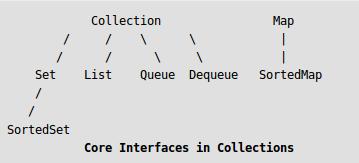
\includegraphics[width=%
0.6\textwidth]{MapInterface}
\end{center} 

\noindent \textbf{GENERICS}\newline
<? extends classe> rappresenta un tipo. \newline
<? extends E> \newline
\textit{SOTTOTIPO} = 1) sei una sottoclasse (extends) 2) sei una sottointerfaccia (implements)
\newline


ArrayList ha come superclasse abstract arrayList. ArrayList implementa collection, quindi ne è sottotipo ma non sottoclasse.
\newline


La \textit{SUBSUMPTION} non funziona tra GENERICS. Per il parametro stesso c'è subsumption, ma non per le collection. Il tipo con
 il ? accetta sottotipi di parametri.
\newline
TIPO ESTERNO: gode sempre della la subsumption, il tipo interno NO, solo con<? extends E>  \newline

[Invarianza del subtyping]: Se ciò non fosse le assunzioni funzionerebbero anche nel tipo di ritorno e questo rischierebbe la totale spaccatura \newline
Se cosi non fosse in java non verrebbero mai rispettate le regole delle classi. \newline
Java di unico ha che esiste il wildchart (?), che è un modo controllato per risolvere questo problemino. \newline
Prima dei generics (2003/2004) in java si programmava tutto a typecast. Per motivi di retrocompatibilità è possibile programmare in tutti e due i modi. E' comunque consigliato usare la porgrammazione con i \textit{generics}. \newline
Metodi che ritornano un booleano iniziano con sempre come se fossero domande; es: hasNext, isEmpty etc.. \newline
Un iteratore non può essere costruito con un new perchè è un'interfaccia. 



\newpage
